% Titre de la partie
\section[Apprentissage par renforcement]{Optimisation de la ville par apprentissage par renforcement}

%%%%%%%%%%%%%%%%%%%%%%%%%%%%%%%%%%%%%%%%%%%%%%%%
% Première diapo (avec des équations)
%%%%%%%%%%%%%%%%%%%%%%%%%%%%%%%%%%%%%%%%%%%%%%%%
\begin{frame}
	\frametitle{Optimisation de la ville par apprentissage par renforcement}
	\framesubtitle{Quelques définitions}

%\begin{itemize}
%\item état : niveau actuel d'avancement dans la "mission"
%\item agent : personnage central de l'expérience qui à terme fera des actions
%\item environnement : espace dans lequel l'agent va évoluer, ici la caractérisation de la ville ( disposition des bâtiments, leurs caractéristiques... )
%\item récompense : amélioration ou régression de l'avancement de la mission
%\item action : c'est l'action que va réaliser l'agent, il y a une liste d'action définie au préalable
%\item état maximale : mission terminée, ville parfaite / quasiment parfaite
%\item ratio d'exploration : chance de faire une action volontairement ou aléatoirement
%\end{itemize}
\pause
\begin{exampleblock}{Etat}
Niveau actuel d'avancement dans la "mission"
\end{exampleblock}
\pause
\begin{exampleblock}{Agent}
Personnage central de l'expérience qui à terme fera des actions
\end{exampleblock}
\pause
\begin{exampleblock}{Environnement}
Espace dans lequel l'agent va évoluer, ici la caractérisation de la ville ( disposition des bâtiments, leurs caractéristiques... )
\end{exampleblock}
\pause
\begin{exampleblock}{Récompense}
    Amélioration ou régression de l'avancement de la mission
\end{exampleblock}

\end{frame}

%%%%%%%%%%%%%%%%%%%%%%%%%%%%%%%%%%%%%%%%%%%%%%%%
% Deuxième diapo (avec des équations)
%%%%%%%%%%%%%%%%%%%%%%%%%%%%%%%%%%%%%%%%%%%%%%%%


\begin{frame}
	\frametitle{Optimisation de la ville par apprentissage par renforcement}
	\framesubtitle{Quelques autres définitions...}
\pause
\begin{exampleblock}{Action}
    Action que va réaliser l'agent, choisie dans une liste d'action définie au préalable
\end{exampleblock}
\pause
\begin{exampleblock}{Etat maximal}
    Mission terminée, ville parfaite / quasiment parfaite
\end{exampleblock}
\pause
\begin{exampleblock}{Ratio d'exploration}
Chance de faire une action volontairement ou aléatoirement
    
\end{exampleblock}
\end{frame}


%%%%%%%%%%%%%%%%%%%%%%%%%%%%%%%%%%%%%%%%%%%%%%%%
% Troisième diapo (avec des équations)
%%%%%%%%%%%%%%%%%%%%%%%%%%%%%%%%%%%%%%%%%%%%%%%%


\begin{frame}
	\frametitle{Optimisation de la ville par apprentissage par renforcement}
	\framesubtitle{Princtipe de fonctionnement}
\begin{figure}
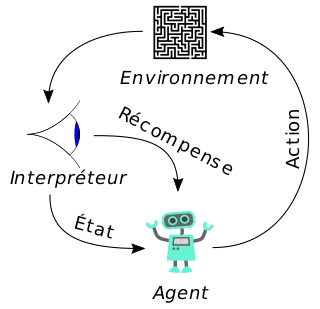
\includegraphics[scale=.4]{diapo/Fig05.png}\\
\caption{Principe de fonctionnement de l'apprentissage par renforcement}
\end{figure}
\end{frame}

